\documentclass[11pt, a4paper, twoside]{article}
\usepackage{graphicx}
\usepackage{amsmath}
\usepackage[margin=0.8in]{geometry}
\usepackage{listings}
\usepackage{float}
\usepackage{fancyhdr}
\usepackage{indentfirst}
\usepackage[inline]{enumitem}
\usepackage{tabularx}
\usepackage{xcolor}
\usepackage{array}
\usepackage{minted}
\usemintedstyle{tango}
\usepackage[belowskip=0pt,aboveskip=0pt,font=small,labelfont=small]{caption}
\captionsetup{width=\linewidth}
\setlength\intextsep{0pt}
\graphicspath{{Plots/}}
\setlist[itemize]{noitemsep, topsep=0pt}
\fancyhead[RO,LE]{EE2703: Assignment 8}
\fancyhead[LO,RE]{Akilesh Kannan}
\cfoot{\thepage}

\title{EE2703: Assignment 8}
\author{Akilesh Kannan (EE18B122)}
\date{\today}

\pagestyle{fancy}

\begin{document}
\maketitle

\section{Introduction}
In this assignment, we shall look at DFTs, using the \texttt{numpy.fft} toolbox.

\section{The Accuracy of the \texttt{numpy.fft} Package}
    To check how powerful and accurate the package is, we shall take the DFT of a sequence of random numbers, then take it's IDFT and compare the two, as to how close they are. This is done using the commands \mintinline{python}{np.fft.fft} and \mintinline{python}{np.fft.ifft}. We also have to use \mintinline{python}{np.fft.fftshift} to shift the $[\pi, 2\pi]$ portion of the DFT to the left as it represents negative frequency, i.e., $[-\pi, 0]$.
    
    The following piece of code accomplishes this task:
    \inputminted[breaklines, linenos]{python}{Code/1.py}
    
    The error came out to be of the order of $10^{-15}$. When the two sequences \mintinline{python}{xOriginal} and \mintinline{python}{xComputed} are plotted together, this is the result:
    
    \begin{figure}[H]
        \centering
        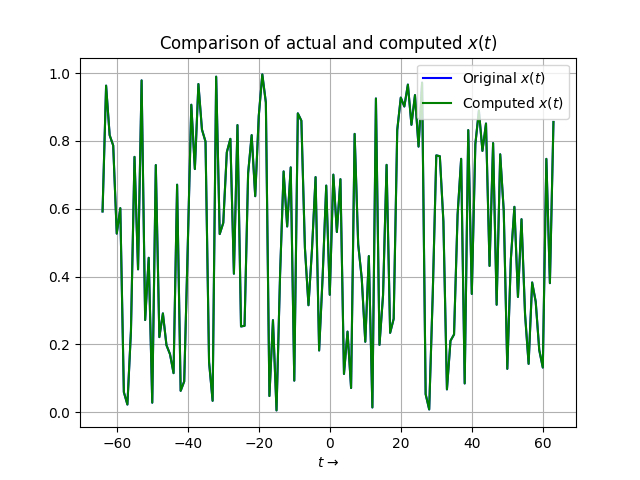
\includegraphics[scale=0.53]{Fig0.png}
        \caption{Comparison of the true and computed values of the random sequence}
        \label{fig:fftRandom}
    \end{figure}
    
    The two sequences overlap and cannot be differentiated !! This shows that the \texttt{numpy.fft} package is very accurate.

\section{Spectrum of $sin(5t)$}
    We calculate the DFT of $f(t)$ by the method mentioned in the above section. Then, we plot the phase and magnitude of the DFT and the following is obtained for $sin(5t)$:
    \begin{figure}[H]
        \centering
        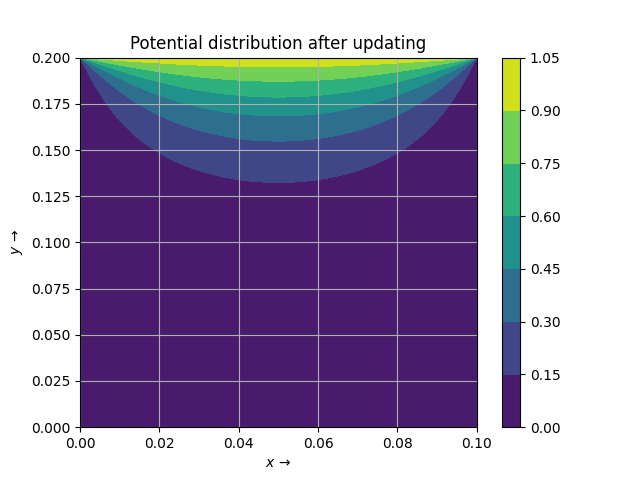
\includegraphics[scale=0.53]{Fig1.png}
        \caption{Spectrum of $sin(5t)$}
        \label{fig:sin5t}
    \end{figure}
    
    This is expected, because:
    \begin{equation}
        sin(5t) = \frac{1}{2j}(e^{5jt}-e^{-5jt})
    \end{equation}
    
    So, the frequencies present in the DFT of $sin(5t)$ are $\omega = \pm5\ rad/sec$, and the phase associated with them is $\phi = \pm \frac{\pi}{2}\ rad/sec$ respectively. This is exactly what is shown in the above plot.

\section{Amplitude Modulation with $(1+0.1cos(t))cos(10t)$}
    We have,
    \begin{equation}
        (1+0.1cos(t))cos(10t) = \frac{1}{2}(e^{10jt}+e^{-10jt}) + 0.1\cdot\frac{1}{2}\cdot\frac{1}{2}(e^{11jt} + e^{-11jt} + e^{9jt} + e^{-9jt})
        \label{eqModAmp}
    \end{equation}
    
    Writing $(1+0.1cos(t))cos(10t)$ in a different form as shown in \eqref{eqModAmp}, we observe that the frequencies present in the signal are $\omega = \pm 10\ rad/sec$, $\omega = \pm 11\ rad/sec$ and $\omega = \pm 9\ rad/sec$. Thus we expect the DFT also to have non-zero magnitudes only at these frequencies.
    
    Plotting the DFT using the \texttt{numpy.fft} package, we get:
    \begin{figure}[H]
        \centering
        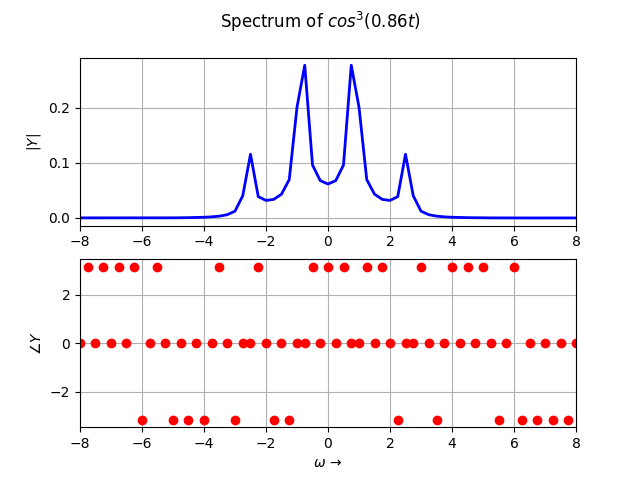
\includegraphics[scale=0.55]{Fig2.png}
        \caption{DFT of $(1+0.1cos(t))cos(10t)$}
        \label{fig:ampMod}
    \end{figure}
    
    Figure \eqref{fig:ampMod} is in line with the theory we have discussed above.

\section{Spectra of $sin^3(t)$ and $cos^3(t)$}
DFT Spectrum of $sin^3(t)$:
\begin{figure}[H]
    \centering
    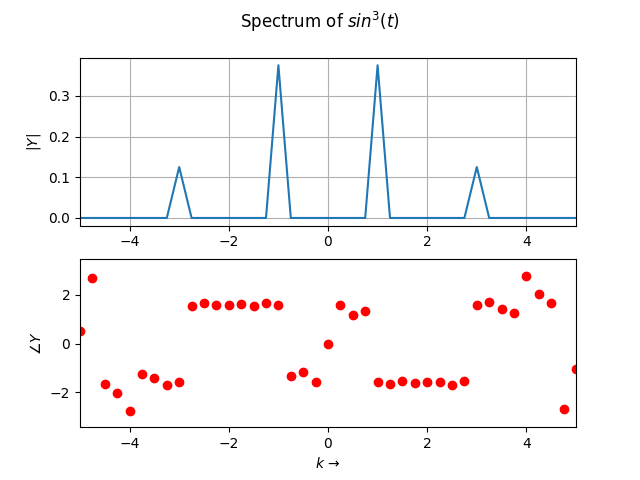
\includegraphics[scale=0.5]{Fig3.png}
    \caption{Spectrum of $sin^3(t)$}
    \label{fig:sin^3t}
\end{figure}

DFT Spectrum of $cos^3(t)$:
\begin{figure}[H]
    \centering
    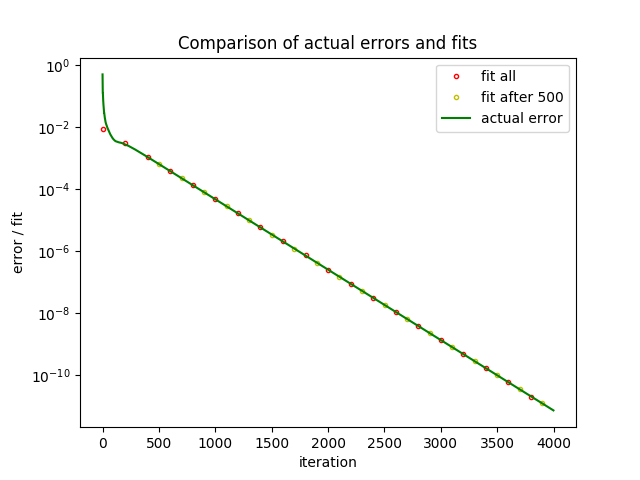
\includegraphics[scale=0.5]{Fig4.png}
    \caption{Spectrum of $cos^3(t)$}
    \label{fig:cos^3t}
\end{figure}

The above 2 figures are expected because:
\begin{gather}
    sin^3(t) = \frac{3}{4}sin(t) - \frac{1}{4}sin(3t)\\
    cos^3(t) = \frac{3}{4}cos(t) + \frac{1}{4}cos(3t)
\end{gather}

So, we expect peaks $\omega = \pm 1\ rad/sec$ and $\omega = \pm 3\ rad/sec$.

\section{Frequency Modulation with $cos(20t + 5cos(t))$}
The DFT of $cos(20t + 5cos(t))$ can be seen below:
\begin{figure}[H]
    \centering
    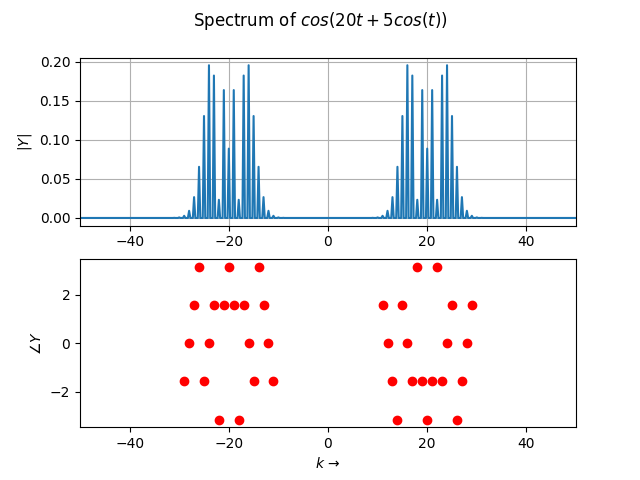
\includegraphics[scale=0.41]{Fig5.png}
    \caption{DFT of $cos(20t + 5cos(t))$}
    \label{fig:freqMod}
\end{figure}

When we compare this result with that of the Amplitude Modulation as seen in Fig \eqref{fig:ampMod}, we see that there are more side bands, and some of them have even higher energy than $\omega = \pm 20 \ rad/sec$.\footnote{J. M. Chowning, \textit{The synthesis of complex audio spectra by means of frequency modulation}, Journal of the Audio Engineering Society, Vol. 21, No. 7, pp. 526-534, \textit{1973}}

\section{DFT of a Gaussian}
The DFT of a gaussian is also a gaussian, as shown below:
\begin{figure}[H]
    \centering
    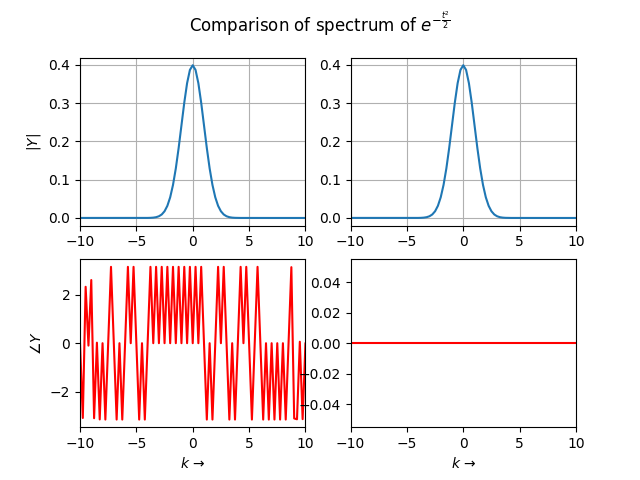
\includegraphics[scale=0.5]{Fig6.png}
    \caption{Gaussian Spectrum}
    \label{fig:gauss}
\end{figure}

\section{Conclusion}
We have thus found out the DFT's of various signals using the \texttt{numpy.fft} package. We need to use the \mintinline{python}{numpy.fft.fftshift()} and \mintinline{python}{numpy.fft.ifftshift()} methods to fix distortions in the phase response.
\end{document}
